\subsection{NGScopeClient}
	Once the data is gathered from the hardware it needs to be presented in a readable manner. to do this we originally planned to build our own front end application. Bryant has experience in that and we did not know of any open source front ends that we liked. However, during Jeremy's hardware research he spoke extensively with an engineer in the feild who happened to mention ngscopeclient.org to him. When we saw it, we were sold. It is an open source platform that works acrossed OSX, Windows, and Linux. It can be interacted with using a C/C++ backend and it has beutiful graphics as shown in figure 2. These features fit our application perfectly.
	
		\begin{figure}[H]
		\centering
		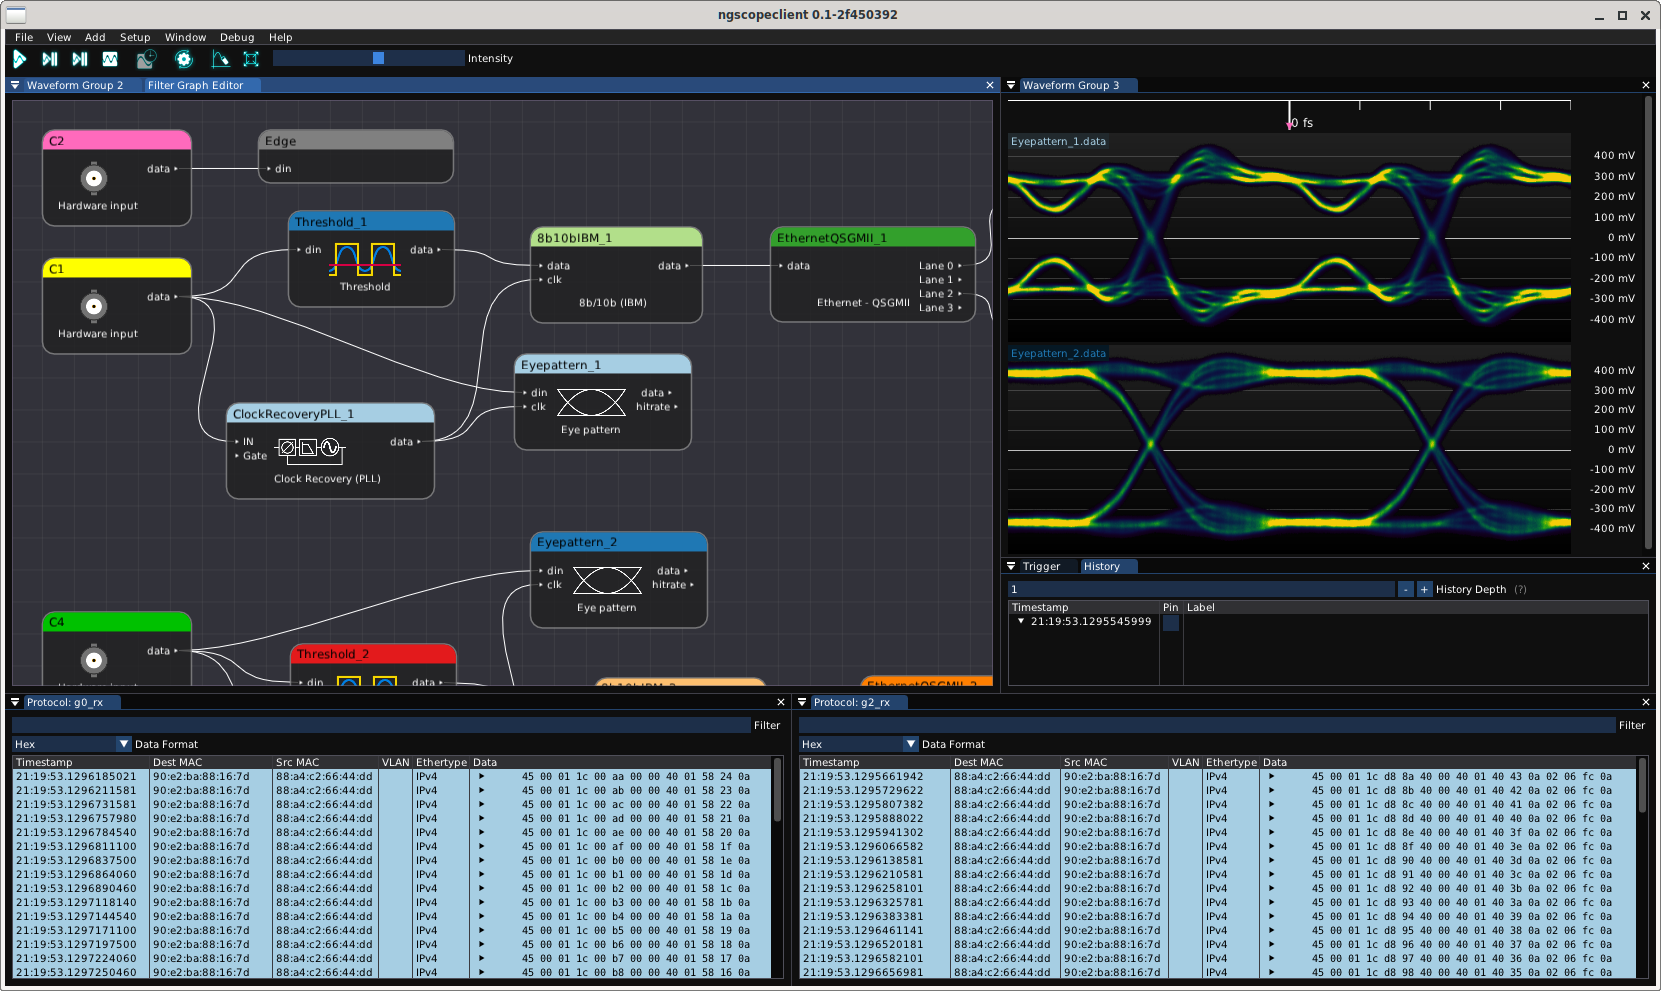
\includegraphics[width=0.8\linewidth]{images/ngscopeclient-intro.png}
		\caption{NGScopeClientGraphics [1]}
		\label{fig:ngscope-client}
		\vspace{15px}
	\end{figure}
	

	‌